\chapter{Current state analysis}
\label{chapter:current-state} 

This chapter presents the analysis on the initial state of the case company. It starts by defining the metrics selected to represent the state of knowledge sharing and
maintenance process and after that, continues by presenting the initial values for these metrics.

\section{Measuring the maintenance process}
\label{section:measuring}

The main topic for the second interview was to identify the key metrics that represent the situation and could be used to measure the change after the implementation phase.
The interview was prepared by finding general software maintenance metrics from the literature (see section \ref{section:literature-metrics}) in addition to custom defined metrics specifically designed for QOCO's
context.

\subsection*{Custom created metrics}

In addition to metrics from literature, also custom created metrics specific for QOCO's challenges were added to the discussion.
These metrics are more suitable for
QOCO as they are specially created for the context, rather than being general metrics. This also means that their validity needs to be carefully addressed to ensure that they work as intended. These custom metrics are presented below.

\emph{Projects per person} - The average amount of projects on different skill levels a single person can contribute to. This works as a measure of knowledge sharing as a higher amount
of projects means better knowledge sharing and wider group of employees who can handle different maintenance tasks.

\emph{Persons per project} - The average amount of persons on different skill levels for a typical project. In addition to measuring the amount of projects, it is necessary to also measure
the amount of persons for different projects to analyze how much skill sets overlap between persons. For example a high number of projects per person, but a low number of persons per project
could indicate that there are some projects that are relatively well known by many people, but also some that are relying on certain key persons.

\emph{Knowledge sharing barriers} - A measure of the most and least significant barriers for knowledge sharing. This gives an idea about the main factors preventing knowledge sharing
and their significance, but on the other hand, also information about which barriers are not an issue at QOCO. This is important to measure since knowledge sharing was considered a major
problem in the initial state, but there was no clear idea about the significance of individual barriers. The evaluated barriers are presented in section \ref{section:barriers}.

\emph{Tickets by type} - Amount or ratio of tickets by their types. Freshdesk has seven different types defined, including info, question, request, change request, alert, incident and problem.
Especially interesting is the amount of actual incidents (alert, incident, problem) in comparison to informative and request tickets, because it represents the true load of maintenance
tasks that actually might require fast response with development activities. These are especially interesting due to initial thoughts about the challenges between development and maintenance
processes.

\emph{Amount of preventable tickets} - The amount of tickets that could have been prevented before a customer needs to report them. Measuring this directly is difficult as there is no general
definition for a preventable ticket, but it is still an important factor since an increasing number of preventable tickets could mean lower customer satisfaction. As a proxy for measuring
preventable tickets, tickets by type could be used with a focus on \emph{ratio of alert tickets}. Higher ratio of alerts out of total tickets would mean earlier reaction without the need to wait
for the customer to report the incidents. This is not exactly the same as the amount of preventable tickets, but it works as a proxy quite well.

\emph{Tickets that actually belong to QOCO} - Amount or ratio of tickets that require actions from QOCO rather than being related to some third party system. This is an interesting measure
as there are several third party systems that QOCO has developed integrations to, but does not have the maintenance responsibility on the system itself. Still a considerable amount of tickets
related to those systems are reported to QOCO causing unnecessary work on QOCO's side, when there is nothing that can actually be done for the ticket. Lower amount of these tickets would mean
better communication of QOCO's responsibilities towards customers and would increase productivity of the maintenance process.

\emph{Time to production} - Time required for a ticket resolution to actually reach production as there are some tasks that can not be deployed to production directly, even though they have
been resolved. Lower time would mean faster actual resolution times correlating with better customer satisfaction, but also reducing the amount of multitasking since already resolved tickets
do not require additional focus in the future.

\emph{Development speed} - There is no single metric that would always be applicable to measure the development speed, but finding the right metrics
for the case company would be beneficial to be able to measure the actual effects of maintenance tasks on development process. However, there are no such metrics used at QOCO currently so measuring the initial state
of development speed is impossible, but it is still worth considering as a point for improvement.

\emph{Waiting for customer} - The time that the tickets are waiting for customer reply over the total resolution time. This metric represents communication issues with the customer
mainly due inactivity on the customer side. It would help to identify whether long resolution times are actually an internal or an external problem.

\emph{Waiting for a third party} - Similarly to previous metric, this measures the time ratio of waiting for a third party over the total resolution time. This also helps to identify external
issues with communication to third parties and clarifies whether issues are internal or external.

\subsection*{Selected metrics}

The presented metrics were carefully evaluated during the second interview, which purpose was to identify the main focus points for improvement and the most critical metrics to measure the
effectiveness of the implementation. The selected metrics can be divided into two categories: maintenance knowledge metrics and process metrics.

First of all, three metrics were selected to measure maintenance knowledge: \emph{projects per person}, \emph{persons per project} and \emph{knowledge sharing barriers}.
These were considered important as one
of the main issues identified already in the first interview was sharing knowledge about maintenance of different projects, which was highly concentrated on key persons. However there was no
clear understanding of the barriers that actually prevent sharing and therefore adding knowledge sharing barriers as a metric is essential. All of the three metrics can also be used to
measure the effectiveness of the implementation since success should be visible as a higher amount of projects for each person with a wider distribution of skill sets at the same time. Also the most
significant barriers should also be lowered if not entirely removed after the implementation while not presenting any new barriers to the organization.

The most important factors of improving the process was identified to be reducing \emph{tickets from unofficial sources} and increasing the \emph{ratio of alerts} out of total tickets to
enhance the ability to recognize and resolve tickets before customers needs to report them to QOCO. Additionally \emph{average resolution time} was considered as an important general metric
that should be kept within reasonable limits, but the main focus was not to aim for faster resolution rates as SLA violations were not an issue. \emph{Waiting for third party or customer}
was also a metric that raised interests, but after a discussion it was evident that access to data about it would be problematic and thus they were left out of focus.

To measure multitasking, a decision to use time tracking data about different \emph{projects and time entries per day} was made. These metrics generally represent the amount of context switching
on average for different persons and teams and thus help to identify whether the problem is team specific or more general. An additional idea was to measure \emph{maintenance hours ratio}, but the
dataset was not sufficient for that purpose. The idea of that would have been to measure the actual ratio between maintenance and development activities, which would represent the
relationship between maintenance and development, but there was no reliable way to measure it and thus it was left out of focus.

\section{Findings}
\label{section:findings-before}

The initial state analysis utilized three data collection methods to identify the challenges. Next the most important findings from each method are presented together
with analysis on the causalities and implications behind the data.

\subsection{Findings from the knowledge sharing survey}
\label{section:survey-results-before}

The initial state analysis phase began with conducting a knowledge sharing survey as knowledge sharing was identified as a challenge during the first interview. The survey consisted of
two main questions: knowledge about several projects that QOCO has implemented throughout its history and an opinion on knowledge sharing barriers. The detailed survey description
is presented in appendix \ref{appendix:survey}. The survey was distributed utilizing Google Forms and a company-wide Slack channel to reach the whole organization. The response
rate was significantly high as 12 out of 15 persons responded to the survey. Two persons were out of office during the whole survey period and one person did not respond at all
(additionally one person was the researcher, who also did not respond to avoid bias). Expertise level of respondents was evenly distributed with four juniors, four seniors and four
executives. The sample is quite representative as the distribution is quite close to the actual expertise level distribution of the organization, although it is notable that there are
four executives in total at QOCO so they are a bit overrepresented in the data. Also work experience distribution that is presented in figure \ref{fig:work-experience-before} is close to
that of the population's since the company has more than doubled its size during the last two years, which can clearly be seen in the graph.

\begin{figure}[ht]
  \begin{center}
    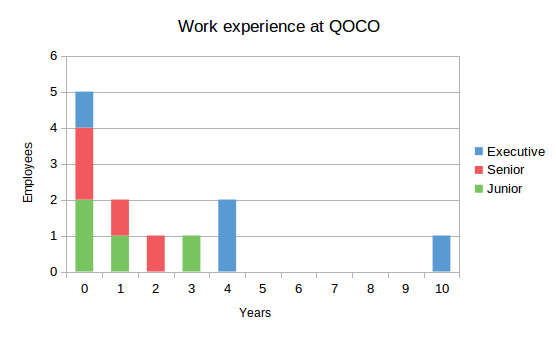
\includegraphics[width=0.9\textwidth]{images/work-experience-before-2.png}
    \caption{Work experience of respondents at QOCO}
    \label{fig:work-experience-before}
  \end{center}
\end{figure}

\subsubsection*{Project knowledge}

The question about project knowledge introduced six levels of knowledge with different scores ranging from zero to five:

\begin{enumerate}
	\itemsep0em % Item separation
	\setcounter{enumi}{-1}
	\item \begin{center} No knowledge at all \end{center}
	\item \begin{center} Knowledge about the business case \end{center}
	\item \begin{center} Knowledge about the business case and general architecture \end{center}
	\item \begin{center} Able to do minor tasks \end{center}
	\item \begin{center} Able to do major tasks \end{center}
	\item \begin{center} Detailed knowledge about the whole project \end{center}
\end{enumerate}

Skill levels can also be combined together. For example level 3+ means levels three to five, so basically an ability to do at least minor tasks on the project.
Combining levels helps to discuss about the differences between skill sets and projects and thus the notation is used in the upcoming sections.

For the projects question, the best known projects were unsurprisingly those that have been developed lately and discussed informally during lunch and coffee breaks. For example
the best known project was MROTools.io with an average knowledge of 2.8 and five persons able to do at least major tasks related to it. This was unsurprising as it has been
a hot topic in discussions and has been developed entirely during the last 1.5 years with a team of four persons dedicated to it. Another example is the second best known project,
Airline 1 technical operations digitalization project with an average knowledge of 2.1. It has also been going on for several years now, but it still
has had quite much development interest of Airline 1 development
team lately and is therefore quite well known by many developers. It can be argued that clearly having company interests on some project and discussing about it formally and informally
on a daily or weekly basis helps to share the knowledge and introduce new persons to the project.

The difference between the most well known and the least known projects is quite significant. For comparison, the least well known project at QOCO is an old legacy project, with an average
knowledge of 0.5 and only one person who knows anything more than just the business case. This is quite typical profile for several legacy projects that have been developed
years ago by the CTO himself with possibly some employees who are no longer working at QOCO. There are still some maintenance tasks related to these projects also and there is on average
only one person who can do anything about them, which is definitely a challenge for the maintenance process and a risk for the company. However it is also important to note that
supporting legacy projects is not the main source of income for the company and thus having too much effort on them can reduce the capability to deliver new projects.

In addition to listing the most and least known projects, the more important aspect about project knowledge was identified to be average knowledge about projects for each
expertise level and an average skill distribution for a typical project. A hypothesis from the interviews with executives was that the executives have significantly more knowledge
about projects than juniors and seniors (H1), who do not have much difference between them (H2). Also it was assumed that usually juniors and seniors know only zero to two projects in detail,
depending on years of experience at QOCO (H3). For the skill distribution, a hypothesis was that there is usually only one to two persons that can do at least major tasks
on the project (H4), while most of the personnel hardly know the business case (H5).

The results of analyzing the project knowledge by different expertise and skill levels are presented in table \ref{table:projects-per-level-before}.
By analyzing these results it is evident that H1 holds, since the executives have a level five knowledge for 9.3 projects on average, which
is much higher than 1.0 of juniors and seniors, which also fulfills H2. The gap is a bit smaller on 3+ level, where juniors have 5.5 projects on average compared to 3.0 of
the seniors. This is explained by longer experience at QOCO on average and different roles, since a product team of EngineData.io consists of seniors whereas Airline 1
development team with several active projects has junior developers for example. This also fulfills H3 as it seems like years of experience at QOCO affect more to project knowledge
than the level of expertise. It is still notable that the executives have 11.8 projects on average with a skill level of 3+, which is more than twice the amount of juniors.
This gap means that many of the tasks related to less known projects fall for the executives who are already busy with many other tasks and new sales at the same time.

\begin{table}[H]
	\begin{center}
		\begin{tabular}{|c|c|c|c|}
			\hline
            	 		& \textbf{Junior} & \textbf{Senior} & \textbf{Executive} \\ \hline
			\textbf{5}  & 1.0             & 1.0             & 9.3                \\ \hline
			\textbf{3+} & 5.5             & 3.0             & 11.8               \\ \hline
			\textbf{1+} & 14.5            & 9.8             & 22.8               \\ \hline
		\end{tabular}
		
		\caption{Average amount of projects at skill level}
		\label{table:projects-per-level-before}
	\end{center}
\end{table}

Analyzing the typical skill distribution for an average project is interesting since it represents the division of skill sets over different projects that is not present
on expertise and skill level analysis. The typical distribution presented in figure \ref{fig:skill-distribution-before} is extrapolated from 12 survey responses to cover
the whole organization of 16 people so it might not be entirely accurate, but the message is still quite clear. From the distribution we can state that there are usually
approximately 2.4 persons with 4+ knowledge on a certain project, so the actual amount is a bit higher than initially estimated with H4. In addition to that, there are
approximately 3.2 persons with 3+ knowledge, which most likely means CTO, COO and some third person depending on the project. Even though H4 does not hold, H5 still does
since in most cases more than half of the organization does not even know the business case of the project. Of course as this is just an average of all projects, there is
a significant difference between older legacy projects and newer projects that are being developed constantly.

\begin{figure}[ht]
  \begin{center}
    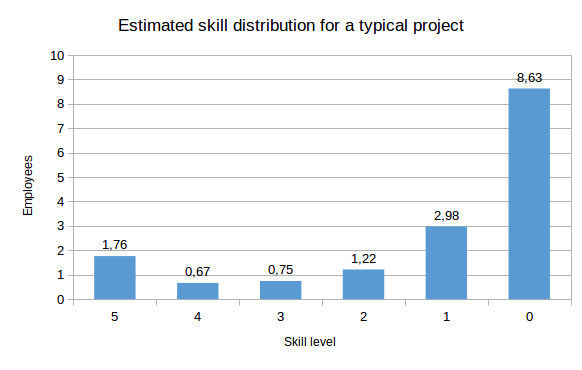
\includegraphics[width=0.9\textwidth]{images/skill-distribution-before-2.png}
    \caption{Estimated skill distribution for a typical project as of February 2019}
    \label{fig:skill-distribution-before}
  \end{center}
\end{figure}

The overall distribution looks promising in a sense that there is potential for knowledge sharing from 3+ level to lower levels since there is for example
on average 1.2 persons already familiar with the business case and architecture. This could help to share some of the workload from CTO and COO to other employees so that
the executives could focus on more important tasks. The fact that half of the organization does not even know the business case of a certain project is not
necessarily a thing to worry about, since considering the ability to contribute to a project by completing tasks, there is not much difference between levels zero and one.
The problem of tasks piling up on executives is not solved by introducing new persons only to the business case.

\subsubsection*{Knowledge sharing barriers}

The second main question was about opinions on significance of different knowledge sharing barriers at QOCO. The opinion was presented using a 5-step Likert scale \citep{Boone2012} with
opinions from \emph{Strongly disagree} to \emph{Strongly agree} for each barrier. 20 barriers were evaluated in total to find out the main knowledge sharing barriers, but also
those barriers that are not an issue at QOCO. The initial hypothesis from two interviews with the managers was that lack of time and resources would be
the biggest challenge together with multitasking (H6). This was assumed by a mutual understanding that schedule had been quite tight on several projects with multiple
concurrent development streams constantly active. Another hypothesis was based on an overall feeling of the company culture and team spirit that was assumed to be strong
and thus should not be experienced as a significant knowledge sharing barrier (H7).

The most significant knowledge sharing barriers are presented below together with their scores. The score was calculated by taking a sum of positive votes for each barrier, ie.
+1 for \emph{agree} and +2 for \emph{strongly agree}. As can be seen, H6 clearly holds since tight schedule and multitasking were considered to be the two most significant
knowledge sharing barriers. A notable barrier is also lack of informal documentation with a score of seven. This represents the situation that most of the knowledge is tacit
knowledge of the CTO and COO, which is not documented anywhere. On the other hand, lack of formal documentation was not considered a significant barrier, which represents
the agile culture of QOCO, since formal documentation does not fit exactly well in agile frameworks. Other significant barriers were also the complex domain of aviation industry and
strong code ownership. The domain is a barrier that can not be entirely solved as QOCO is focused on aviation industry and knowledge about it is learned through years of experience.
Code ownership on the other hand reflects the results of project knowledge question as the code ownership of especially legacy projects is usually at the hands of the CTO and therefore
it could be solved with similar solutions that are aimed to share the knowledge of different projects from the executives to other employees.

\begin{center}
	The most significant knowledge sharing barriers at QOCO:
	
	\begin{enumerate}
		\centering
		\item Tight schedule (15)
		\item Multitasking (10)
		\item Lack of informal documentation (7)
		\item Complex domain (6)
		\item Strong code ownership (6)
	\end{enumerate}
\end{center}

The other end of the scale is the least significant knowledge sharing barriers and as can be seen from the list below, H7 holds quite well. The list was constructed
similarly by giving score of +1 for \emph{disagree} and +2 for \emph{strongly disagree}. The barriers related to
organizational culture are considered as least significant at QOCO and therefore it can be stated that the overall culture of QOCO is open for discussion and supportive towards
knowledge sharing even though \emph{organizational culture} itself did not make it to the list with a score of seven. It is evident that the employees have high motivation and
trust on each other, which is required to share knowledge in the first place. It is good to see that the main challenges of knowledge sharing are not related to attitudes and
organizational culture, that are harder to solve than the barriers related to organizing work such as scheduling and multitasking.

\begin{center}
	The least significant knowledge sharing barriers at QOCO:

	\begin{enumerate}
		\centering
		\item Physical work environment (14)
		\item Difference in age (14)
		\item Lack of motivation (13)
		\item Lack of trust (13)
		\item Strong organizational structure (12)
	\end{enumerate}
\end{center}

In addition to the two main questions there was also an additional voluntary question about open thoughts on knowledge sharing challenges at QOCO. The responses reflect
the results of the main questions as one respondent says that ``\emph{... there is very little 'free' time for knowledge sharing unless absolutely necessary}'', which
emphasizes the challenge of tight scheduling as there is no surplus time when all the deadlines are closing in. Also several respondents emphasized the knowledge gap
between the executives and others by stating that ``\emph{those with the most knowledge are also the busiest}'' and
``\emph{key persons such as (CTO) and (COO) have lot of maintenance responsibilities which is a challenge for new business}'' latter of which raises the concern about
the ability to sell new projects due to maintenance tasks that keep these key persons busy. Another point to note about general knowledge sharing is the fact that
``\emph{... the tasks are usually given to the most experienced in each task}'', which effectively prevents knowledge sharing and enforces code ownership that has been
identified as the 5th most significant barrier. One respondent also pointed out the strong team boundary between Airline 1 consulting and development teams since
``\emph{there is little communication between consulting and coding team}'', which is a bit odd considering the fact that they are working for the same customer on similar
projects even though the focus of the tasks is different. Increased communication could clearly benefit both of them.

\vspace{12pt}

% Concluding paragraph

To conclude the findings from the knowledge sharing survey, the company culture is supportive towards knowledge sharing and therefore the focus should be on solving the
tight scheduling and multitasking issues that are considered to be the two most significant barriers. This leads to a situation where many of the maintenance tasks are
solved by the CTO or COO, which effectively prevents knowledge sharing and will not be scalable in the future. To encourage sharing of knowledge some of the maintenance
tasks could be shared to other employees as well even though it might mean increased costs in short term, but this will be necessary considering long term scalability.
By delegating some of the tasks to other employees, the executives could also focus on more important future sales and current development projects that will generate
majority of the revenue in the future.

\subsection{Findings from the first workshop}

The first workshop was organized to identify the issues related to the maintenance process as knowledge sharing was already
addressed with the survey. The workshop was targeted for MROTools and Airline 1 development teams as special interest towards relationship between maintenance and development
was considered important. Additionally the executives and Airline 1 consulting team were invited, but only one person from consulting team and none of the executives
could attend the workshop. However, the topics were later discussed with the executives separately. The results
of the first workshop can be divided into three main categories: process related findings, customer related findings and findings related to the tools being used.

\subsubsection*{Process related findings}

First of all, one of the main challenges of the initial maintenance process was the fact that there was a lot of informal communication outside of the official Freshdesk process.
This is clearly evident on the reaction of the participants when the official model in figure \ref{fig:ticketing} was presented as a boundary object. Comments such as
``\emph{that is a nice model, but it is nowhere near the actual process}'' were presented, which represents clearly how well the official process is adopted internally. This informal
communication via different channels often leads to situations where some of the information has been lost or altered when the issue reaches the person responsible for solving it.
This is problematic since missing information means that the responsible person needs to dig for that either from the customer or colleagues and in the worst case, starts to work
on a completely different problem than was originally reported. There is also a practical problem of billing the hours used for the maintenance task if it is reported by chatting by
the coffee machine rather than actually reporting it to Freshdesk. The problem of informal communication about maintenance tasks is also visible as concentration of the customer interface
around individual persons for each project who then delivers the information forward, if he remembers to do so. This means that if the person will not be available at some times,
the process is essentially broken since the customer does not have anyone to contact in case of issues.

Another internal process related finding was that initially there was no clearly defined person responsible for addressing the issues on Freshdesk when they are reported there.
The initial process was usually that "someone" will address them when they have time, that "someone" usually being the CTO or COO. It was also said that developers do not know
about the time limits on SLA contracts, which makes it rather hard to prioritize maintenance and development tasks among each other. Prioritization of the maintenance tickets
is also relatively difficult as there was no clear policy on different priorities, meaning that most of the tickets were of "low" priority. The main issues of lacking proper internal
prioritization guideline and vaguely defined responsibility on maintenance tasks means that the maintenance tasks will disturb development work by pausing it in the middle of
a flow just to realize that the task is actually of low priority and could be addressed later with a better time slot. These interruptions cause developers to lose their focus
for a while, which slows down the development work and causes inefficiency.

In addition to unclear responsibilities, also the tagging feature in Freshdesk was rarely used. If properly used, it could help tracking issues related to certain project for example,
rather than just having a list of all tickets visible at the same time. This results in inefficient search functionality and causes loss of time when searching for issues related
to own line of work. One additional finding related to the process was about customer satisfaction that is not measured with any actual metric. There have been some interviews
a while ago, but the current understanding of a relatively good customer satisfaction is not based on any tangible metric. Of course it could be argued that the customer would
tell if they were unsatisfied with some aspects, but there is still room for improvement in the current situation. Specified and tracked metrics of customer satisfaction could
help QOCO to react to changes in customer satisfaction faster, resulting in better overall customer experience.

\subsubsection*{Customer related findings}

The root cause for informal communication are the customer's representatives who use several channels for contacting QOCO personnel including, but not limited to, email, phone calls,
Slack and chatting by the coffee machine. The use of these channels then continues on QOCO's side and the task might never be visible on Freshdesk even though it is a clear maintenance
task. Of course QOCO as a small company can not enforce a strict maintenance process since flexibility and customer satisfaction are its main advantages as a small company. If QOCO would
enforce the official maintenance process too strictly, it would be an easy decision to switch partner to some large general software service provider with a similar process, but benefits
of a large corporation. Therefore even though informal communication is problematic and usually initiated by the customer, the solution to it is not trivial and requires careful assessment
of both internal and external processes including customer satisfaction as a highly important factor.

In addition to informal channels being used for communication, also initial requests are usually of low quality and require further clarifications from the customer. Relatively common
issue is that "something is not working" with a screen capture of some system QOCO's developers have never seen. This might be due to technical skills of the end users that are
experiencing the issues, but another point noted in the workshop is that many of the issues are "highly critical" according to the customer, while still lacking information required to 
resolve the issue. It might even be the case that the reporter of the ticket is not available or has no skills required to provide clarifications. When the low quality of initial reports,
informal communication channels and an undefined responsibility of responding to tickets discussed earlier are combined together, it is no wonder that the maintenance process can be
considered as inefficient and causes interruptions on development.

The expectations on response and resolution times are also unbalanced in some cases since the tickets might be waiting for customer reply for a long time, but still the customer
considers every tickets as critical and expects responses and resolutions fast. This causes some of the prioritization and interruption issues mentioned earlier, but also frustration
on developers' side as the ticket might be pending for a long time, but when the information arrives, it suddenly becomes a top priority ticket.

\subsubsection*{Findings on tools being used}

On the tools side, the single most important finding was that QOCO had a plan on Freshdesk that allows five users to be added to the system. This is highly problematic since there are currently 16 employees at the company with at least 12 of them participating in maintenance activities. There has been a habit of rotating the fifth user for the one
in need in each situation, but it is obvious that the official process can not be used by having five licenses for 12 employees. This problem is also only going to get worse in the future
if the company keeps on growing. The limited number of user licenses will further encourage informal communication outside of Freshdesk as not everyone will have access to the information
stored there. Additionally it was also noted that the email client provided by Freshdesk has several usability issues, which will further encourage direct use of informal email
communication outside of Freshdesk.

In addition to the usability issues of the email client, another major drawback on usability is the search functionality that does not allow users to query tickets by their content, which would
be highly beneficial in cases where the ticket title only contains "not working" for example. This makes it hard and time consuming to search for certain tickets and makes the use of
Freshdesk inefficient. This usability issue goes together with missing tags, that could be used for querying. Together these two challenges make it unnecessary difficult to find tickets
and could be beneficial to improve the overall process.

What comes to the challenge of internal prioritization, another challenge in the current process is separation of maintenance and development tickets to two completely different systems:
Freshdesk and JIRA \footnote{https://fi.atlassian.com/software/jira}.
This means that these two systems are often out of sync, which makes organizing and prioritizing work difficult and may cause delays to both maintenance and development tasks.
In addition to internal JIRA, at least Airline 1 development team has customer's own JIRA for higher level issue tracking, which introduces a new problem of synchronizing three separate systems.
Generally having multiple separate systems slows down all processes as the systems need to be manually updated and checked for new updates, which causes unnecessary trouble for the development
teams and should be solved.

\vspace{12pt}

% Concluding paragraph

To conclude the main findings of the first workshop, it could be stated that the old ad hoc process of best effort is still visible as informal communication and customer interfaces that are
concentrated on certain key persons. On the other hand it is also hard to enforce the official model even internally when there are not enough user licenses for each person participating
in the maintenance process. Also ticket quality and proper prioritization should be emphasized as there is currently an unbalanced understanding of priorities as customer tends to consider
everything as highly critical, whereas most of the tickets are classified as low priority on Freshdesk. These are the main points of improvement identified in the workshop.
These should be carefully considered when creating the solution proposals and comparing them with each other.

\subsection{Findings from the data exports}

The last data collection method used in the initial state analysis was analyzing data exports from existing systems, namely ticket tracking system Freshdesk and time tracking system Toggl.
The goal of the data analysis was to find the state of the maintenance process by evaluating several predetermined metrics including the amount of automatic tickets, ticket reporters,
resolution times and context switches.

\subsubsection*{Freshdesk}

Freshdesk data export from 2018 provides information about individual tickets including for example their resolution time and priority. The first interesting factor to measure was the amount
of automatic tickets, ie. alerts, in relation to other ticket types. Distribution of the ticket types is presented in figure \ref{fig:ticket-types-before}. From the graph it is notable that
only 7 \% of tickets are automatic alerts while most of the issues are still reported manually. It has been identified that the amount of alerts in comparison to other ticket types
should be higher since it would mean that the tasks could be resolved already before the customers notice anything. This would mean a better customer experience, but also improve efficiency
of the maintenance process as it is usually easier to track down the source of an alert compared to a manually reported incident.

\begin{figure}[ht]
  \begin{center}
    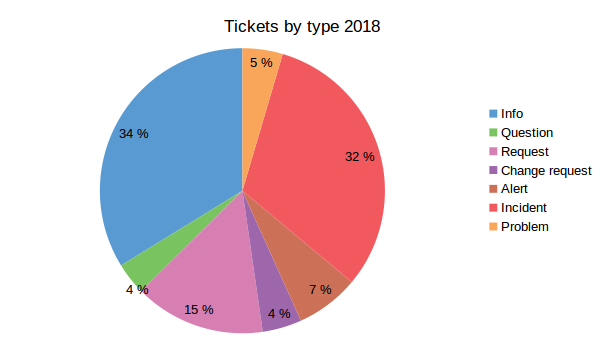
\includegraphics[width=1.0\textwidth]{images/ticket-types-before-2.png}
    \caption{Ticket types, excluding tickets without a type}
    \label{fig:ticket-types-before}
  \end{center}
\end{figure}

The measure of tasks that are reported through informal channels can be approximated by analyzing the reporter of each ticket. In most cases the tickets that are reported internally have
originated through informal channels and have been added to Freshdesk by QOCO's employee meaning that the reporter domain will be qoco. The analysis of the ticket reporter domains
is presented in figure \ref{fig:ticket-domains-before} and it can be seen that approximately 10 \% of all tickets are reported through informal channels. However it is notable
that the whole truth about tasks in informal channels is not visible in Freshdesk tickets as not all of the tickets in informal channels end up as tickets to Freshdesk, which makes
it hard to estimate the actual proportion. From the graph we can also see that only 2 \% of the tickets come from 3rd party vendor that is handling the first level of support for Airline 1.
Basically this means that Airline 1 reports some first level tickets directly to QOCO instead of going through the official process of reporting to the third party vendor, which then escalates the ticket
to QOCO if necessary.

As argued, the changes in reporter domain proportions work as a proxy for estimating the amount of tickets that are reported through informal channels. It needs to be noted that increased proportion of internally
reported tickets could be interpreted as increasing amount of tickets in informal channels, when it actually meant that just larger amount of informal tickets are also reported to Freshdesk,
which naturally is a good thing. Therefore the reporter domains can not be analyzed alone, but they need to be analyzed together with the total amount of tickets, which is presented in figure
\ref{fig:resolution-time-before}.

\begin{figure}[ht]
  \begin{center}
    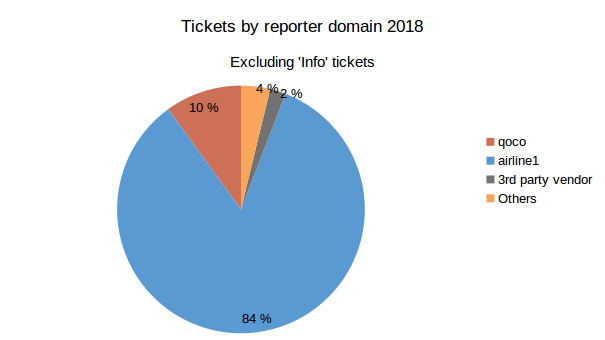
\includegraphics[width=1.0\textwidth]{images/ticket-domains-before-2.png}
    \caption{Tickets by reporter domain}
    \label{fig:ticket-domains-before}
  \end{center}
\end{figure}

One of the most important measures of process efficiency and customer experience is the average resolution time of tickets. This is presented as a monthly average over 2018 in figure
\ref{fig:resolution-time-before} together with the total ticket count to emphasize the relationship between them. The graph includes only low priority tickets, because the few tickets
that were on other priority levels had several hundreds or even thousands of hours in resolution time, meaning that they were exceptions to the general maintenance process. 
As can be seen in the graph, the average resolution time has been in a downtrend throughout 2018, but interestingly there seems to be an upward spike every four months.
There was no clear explanation for these spikes, but each time there seems to be an increase in total ticket amount during the previous month, probably at least partly affecting the
resolution times of the next month as well. Another point to note was that there was also different production deployments and initializations of several systems during those spikes,
which also partly explain longer resolution times. Generally it could be stated that the overall resolution times and total ticket counts have been in a downtrend, which is positive
and should continue similarly in the future as well.

\begin{figure}[ht]
  \begin{center}
    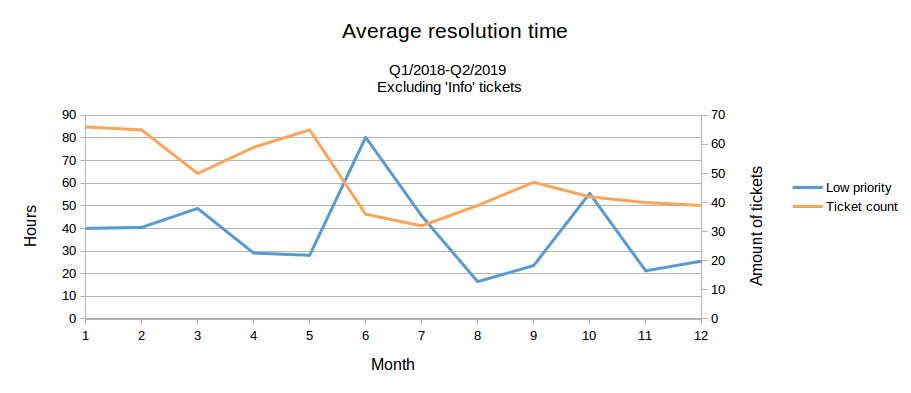
\includegraphics[width=1.0\textwidth]{images/resolution-time-before-2.png}
    \caption{Average resolution time by month}
    \label{fig:resolution-time-before}
  \end{center}
\end{figure}

\subsubsection*{Toggl}

In addition to the ticket data from Freshdesk, there was also time tracking data available from Toggl. Especially interesting aspects about that was to measure the amount of multitasking
and therefore context switches that cause interruptions to productivity. The results of the team based analysis are presented in table \ref{table:toggl-before}.
The table excludes EngineData team since it has been established in January 2019 and thus was not present in the 2018 dataset. The analysis consisted of two metrics: projects per day
meaning the amount of different projects the teams work during the day on average, and the amount of time entries per day each basically representing actual context switches. The dataset
does not include all of QOCO's projects and therefore the values are only approximations of the real values, but they still can be used to compare different teams with each other.

\begin{table}[H]
	\begin{center}
		\begin{tabular}{|c|c|c|}
		\hline
        		              		       & \textbf{Projects / day} & \textbf{Time entries / day} \\ \hline
			\textbf{Airline 1 consulting}  & 1.1                     & 1.4                         \\ \hline
			\textbf{Airline 1 development} & 1.7                     & 3.3                         \\ \hline
			\textbf{Executives}    		    & 1.8                     & 2.4                         \\ \hline
			\textbf{MROTools}         		& 1.1                     & 2.1                         \\ \hline
		
		\end{tabular}
		
		\caption{Average context switches per day}
		\label{table:toggl-before}
	\end{center}
\end{table}

From the table it is notable that the executives and Airline 1 development team tend to multitask more than Airline 1 consulting and MROTools teams. This can be explained by different types of
work as MROTools team focuses on a single SaaS product development and the consulting team handles mainly support tasks that are all grouped under the same project. Airline 1 development team
on the other hand has had many parallel development projects on at the same time, resulting in a higher multitasking factor. To further analyze this challenge, the multitasking factor of Airline 1
development team is analyzed on a monthly basis in figure \ref{fig:dev-team-toggl-before}. It can be seen that the average level
of time entries per day is between 2.5 and 3.5, but during July and August the value has been significantly higher than that. This is alerting as an increased
amount of context switches generally slows down both maintenance and development tasks and therefore it should be considered when proposing solutions
at least for Airline 1 development team.

\begin{figure}[H]
  \begin{center}
    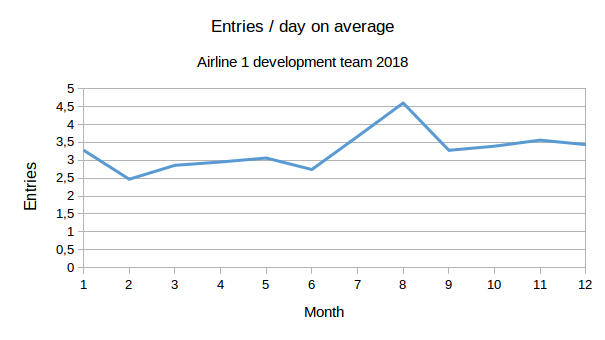
\includegraphics[width=1.0\textwidth]{images/dev-team-entries-before-2.png}
    \caption{Average time entries per day for Airline 1 development team}
    \label{fig:dev-team-toggl-before}
  \end{center}
\end{figure}

To conclude the main findings from the data exports it is evident that the maintenance process is not exactly working as it is supposed to. Even though the resolution times and total ticket
amounts have been generally decreasing, it is alerting that there are still regular spikes on resolution times every four months. Also multitasking seems to be an issue mostly for Airline 1
development team, which lowers the productivity of that team and slows down both development and maintenance processes.